%\documentclass[]{article}
%\usepackage{graphicx}
%\usepackage{subfig}
%\usepackage{amsmath}
%\usepackage{amsfonts}
%\usepackage[margin=1in]{geometry}

%\begin{document}

Now it's time to actually see how well the various algorithms we have discussed performed on our dataset. In table \ref{tab:Classifiers}, we list the performance of various classification algorithms on our dataset. The best performing classifier was an svm that uses the raw data that wasn't reduced in dimensionality. The first 5 rows of the table are all quite comparable in performance, however. 

Although many of the methods used performed quite well with a large amount of training examples used, there was a variability in these model's performance with a smaller amount of training examples used. Most notably, there was a large decrease in performance with a small number of examples using svm pca compared to a large number of examples. L1 regularized logistic regression also performed significantly worse with a small number of data points.

\begin{center}
\begin{table}
\begin{tabular}{lccccl}
\hline
%Name & 50-Mean \% & 50-STD \% & 1500-Mean \% & 1500-STD \% &  description\\
Name & 50-$\mu$ \% & 50-$\sigma$ \% & 1500-$\mu$ \% & 1500-$\sigma$ \% &  desc.\\
\hline
svm & 84.4 & 7.3 & 94.4 & 7.3 & svm with linear kernel\\
ridge & 91.3 & 1.7 & 94.0 & 0.2 & $L_2$ regularized logistic regression\\
lasso pca &  86.4 & 6.1& 94.0 & 0.5 & $L_1$ regularized logistic regression with 50 dim pca\\
svm pca &54.6 & 11.1&  93.3 & 0.2 &  linear kernel svm with 50 dim pca applied first\\
lasso & 73.7& 5.7 & 92.4 & 0.8 & $L_1$ regularized logistic regression\\
naivebayes pca small & 87.5& 2.4 & 90.1 & 0.3  & naivebayes smooth with 5-dim. pca\\
naivebayes & 60.8 & 7.9& 79.0 & 1.8& naive bayes with `add one' smoothing\\
naivebayes pca  & 74.2 & 5.2 & 77.4 & 0.8 & naivebayes smooth with 50-dim. pca\\
naivebayes rand & 55.6 & 3.4 & 67.0 & 2.8  & naivebayes smooth with 50-dim random projection\\
\end{tabular}
\caption{Classifiers}
\label{tab:Classifiers}
\par
\end{table}
\end{center}



One of our motivating objectives is to find sub-regimes of $n << p$. To do this, we subsampled our training set and varied the size of the reduced set. For each size, we performed 10-fold cross validation. In Figure \ref{fig:largecompareAcc}, we plot the accuracy of the various algorithms as a function of the training set size. We weren't able to find any interesting sub-regimes or crossing points, unfortunately. Perhaps our full dataset was too small to begin with, and interesting sub-regimes would have occurred if we had increased rather than decreased the size of the training data. Another reason that perhaps we don't see any interesting sub-regimes is that classification on our dataset is simply too easy and the performance of many of the classifiers is squeezed into the nineties. 

\begin{center}
\begin{figure}[!ht]
\centering
\subfloat[Accuracy]{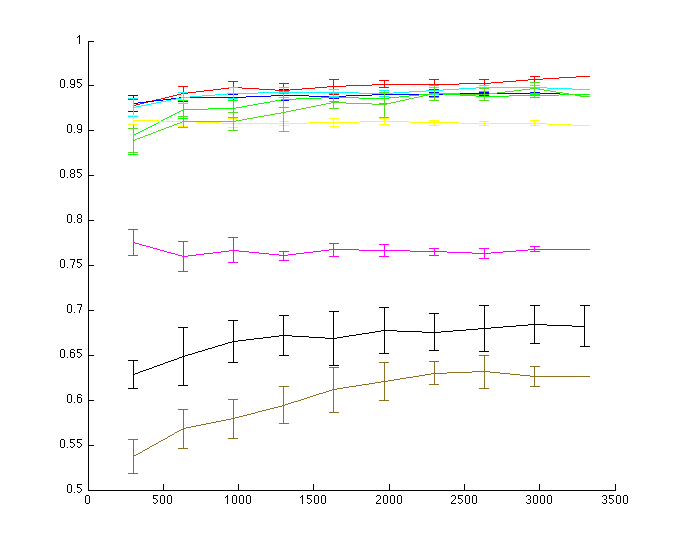
\includegraphics[width=.7\textwidth]{../images/c3.png}}
\subfloat[Legend]{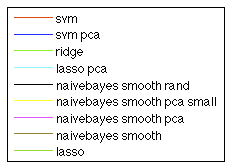
\includegraphics[width=.3\textwidth]{../images/legend.png}}
\caption{Accuracy vs Size of subsampled training data used}
\label{fig:largecompareAcc}
\par
\end{figure}
\end{center}


Overall, one useful a useful outcome of our experiments is that they suggest that sometimes dimensionality reduction is critical when we have little data. To illustrate this phenomenon, in figure \ref{fig:lassoCompare} we vary the size of the training set and compare the accuracy of  $L_1$ regularized logistic regression with and without pca being applied to the data. We find that for extremely small training set sizes, lasso with pca performs substantially better than it does on the raw 17,000 dimensional data. However, as we increase the size of the training set, the performances become comparable. If our dataset had been larger, we would have perhaps identified that the performances cross eventually. 

\begin{center}
\begin{figure}[!ht]
\centering
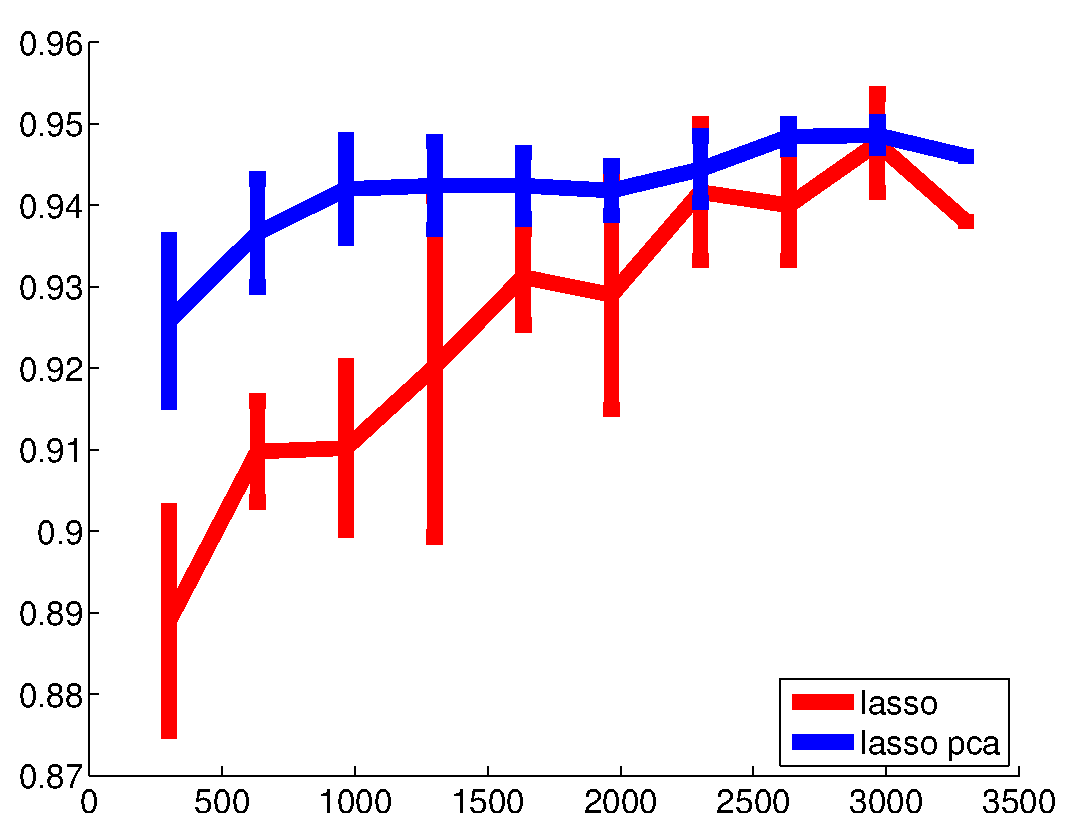
\includegraphics[width=.5\textwidth]{../images/_lasso_lasso_pca_acc.eps}
\caption{Accuracy vs. Train set size}
\par
\label{fig:lassoCompare}
\end{figure}
\end{center}

	In the background section, we discussed an important result due to Ng and Jordan that logistic regression is asymptotically better than naive Bayes, but naive Bayes approaches its higher asymptotic accuracy more quickly ~\ref{jordan2002discriminative}. In figure \ref{fig:LLL}(a), we vary the size of the training set and compare logistic regression with pca and logistic naive Bayes with pca. For this dataset, we are not able to identify a regime of small train set sizes where classification performance for naive Bayes is better. Logistic regression is always superior. One defining characteristic of our dataset, which Ng and Jordan don't account for in their arguments, is the very high level of the data, even after 50-dimensional pca projection (50\% sparse). The number of nonzero observations for each observation is quite low, and thus naive Bayes can not estimate its component-wise Gaussian distributions accurately. Logistic regression makes fewer assumptions about the underlying generative process and consequently less vulnerable to sparsity. 

	We found that dimensionality reduction is important to maintain high classification accuracy for some algorithms in the $n << p$ regime. An additional advantage of it is reduction in time and memory requirements for training. In figure \ref{fig:LLL}(b) we plot the time cost of training a naive Bayes model with pca v.s. a naive Bayes model without pca. We find that the training time for the raw 17,000 dimensional data (red curve) explodes as we increase the training size. Due to the seemingly linear relationship of time vs. train set size for the red curve for most of the train set sizes, its sudden explosion, and the large error bars on the final measurement, it seems like the laptop the experiment was run on became strained and unreliable. When the memory limits of the computer are approached, it suddenly needs to do lots of work to keep things in place, and as a result, runtimes increase tremendously. 


\begin{center}
\begin{figure}[!ht]
\centering
\subfloat[Which of Ng and Jordan's regimes are we in? Accuracy vs. train set size]{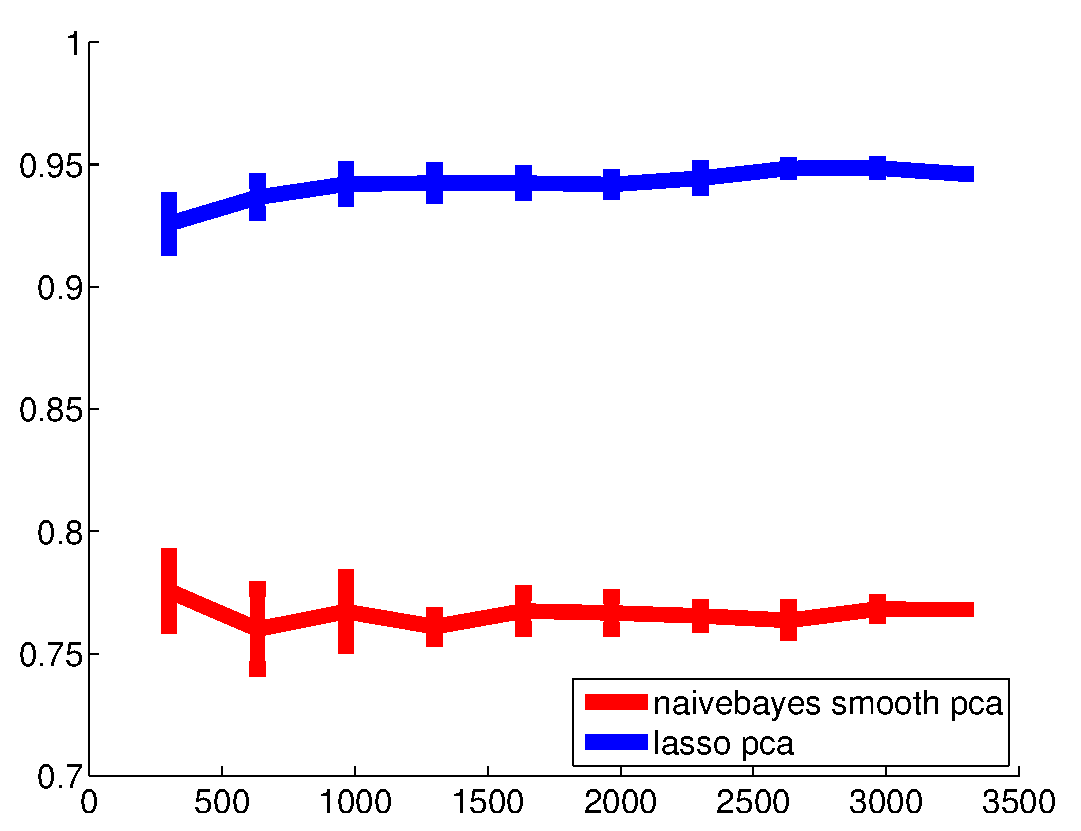
\includegraphics[width=.5\textwidth]{../images/_naivebayes_smooth_pca_lasso_pca_acc.eps}}
\subfloat[NB train time vs. train set size]{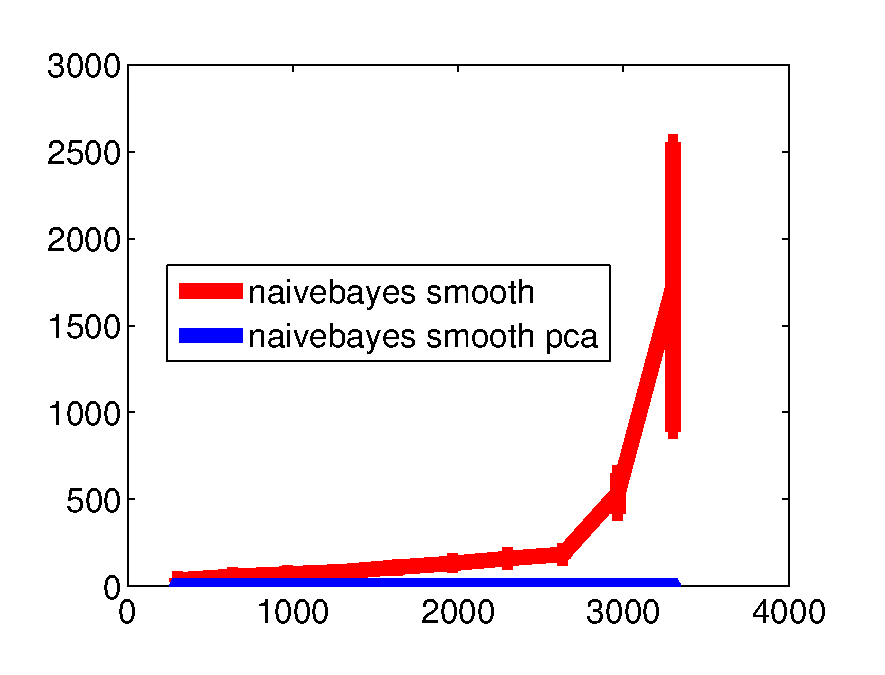
\includegraphics[width=.5\textwidth]{../images/_naivebayes_smooth_naivebayes_smooth_pca_time.eps}}
\label{fig:LLL}
\par
\end{figure}
\end{center}

%\end{document} 

